\chapter{Implementation, Integration and Test Plan}

\section{Implementation plan}
The CKB system will be implemented following a bottom-up approach, taking into account the dependencies between the components within the same subsystem. In this way an incremental integration is promoted, making bug tracking easier because it allows testing of the intermediate outcomes. This strategy allows different teams to work in parallel on implementing different features.

\subsection{Component integration and testing}
This section explains which components are implemented at each stage, as well as how they are integrated and tested. \newline
Since some components may not work in isolation, driver and stub components will be realized to simulate the behaviour of the missing modules. \newline

In the first stage (in figure \ref{fig:stage1}) the Model and the Entity Manager are implemented and unit tested, using a driver for the components that are missing. These components handles all the major functionalities of the system and all the interactions with the database.
\begin{figure}[h]
    \centering
    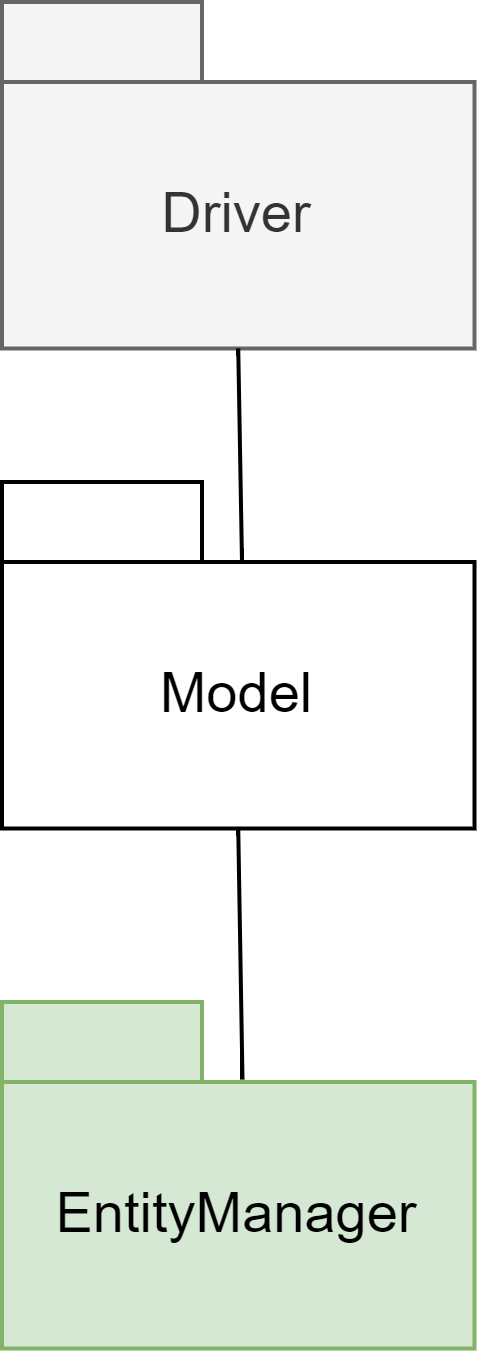
\includegraphics[scale=0.5]{images/testing/stage1.png}
    \caption{Stage 1}
    \label{fig:stage1}
\end{figure}
\clearpage

In the second stage (in figure \ref{fig:stage2}) the components responsible for the sign up and log in of users are implemented, since some components will need this features in the next stage. The Email Manager component is still not implemented and a stub is used to simulate it. 
\begin{figure}[h]
    \centering
    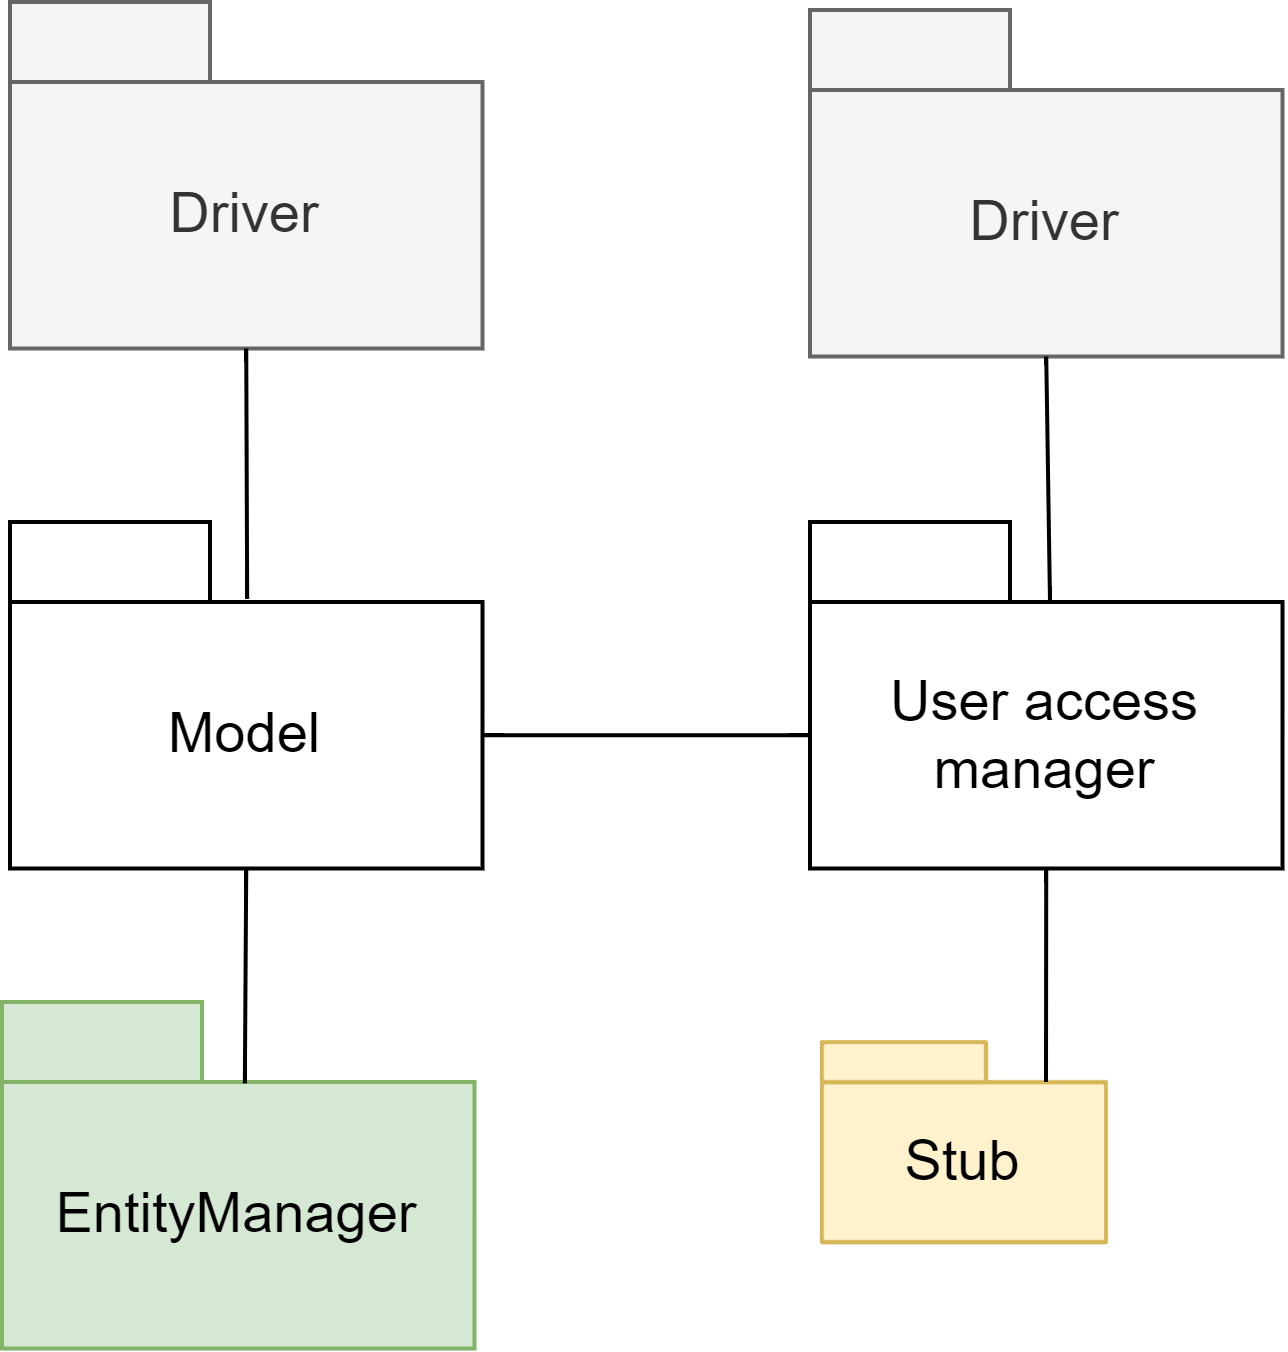
\includegraphics[scale=0.7]{images/testing/stage2.png}
    \caption{Stage 2}
    \label{fig:stage2}
\end{figure}

In the third stage (in figure \ref{fig:stage3}) the components responsible for the creation and management of tournaments and battles are implemented. A driver is used to simulate the interfaces in order to test the new components.  
\begin{figure}[h]
    \centering
    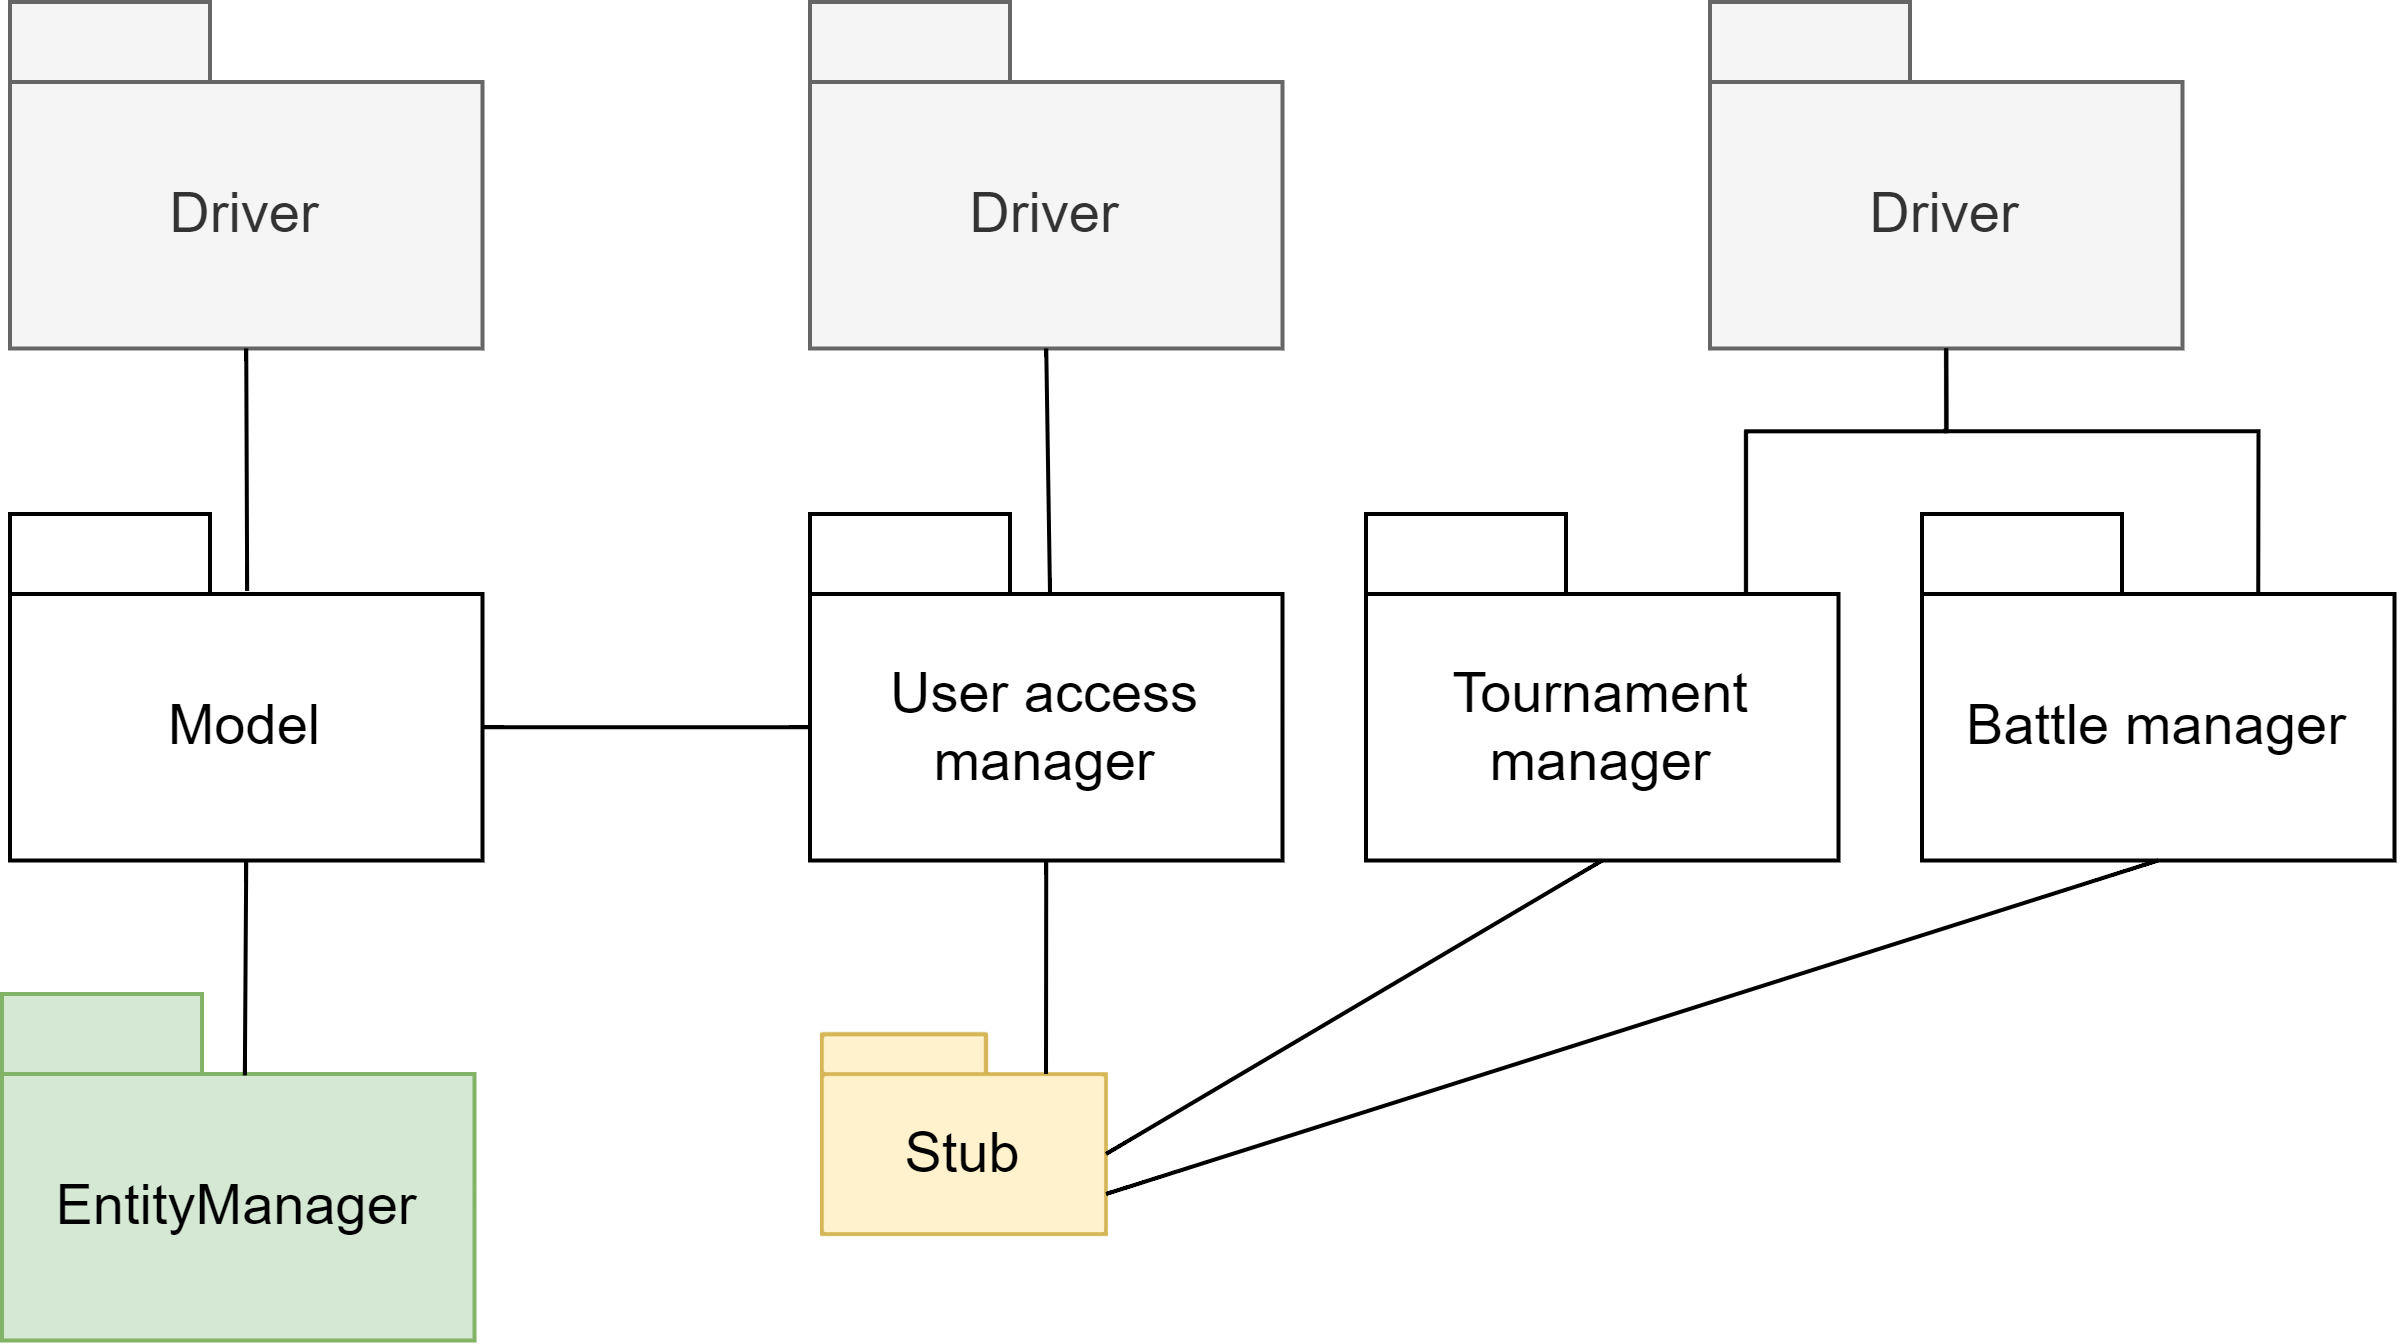
\includegraphics[scale=0.7]{images/testing/stage3.png}
    \caption{Stage 3}
    \label{fig:stage3}
\end{figure}
\clearpage

In the fourth stage (in figure \ref{fig:stage4}) the Automatic Evaluation manager is implemented and another stub is used to simulate the external components (GitHub and static analysis tool API) in order to unit test it.
\begin{figure}[h]
    \centering
    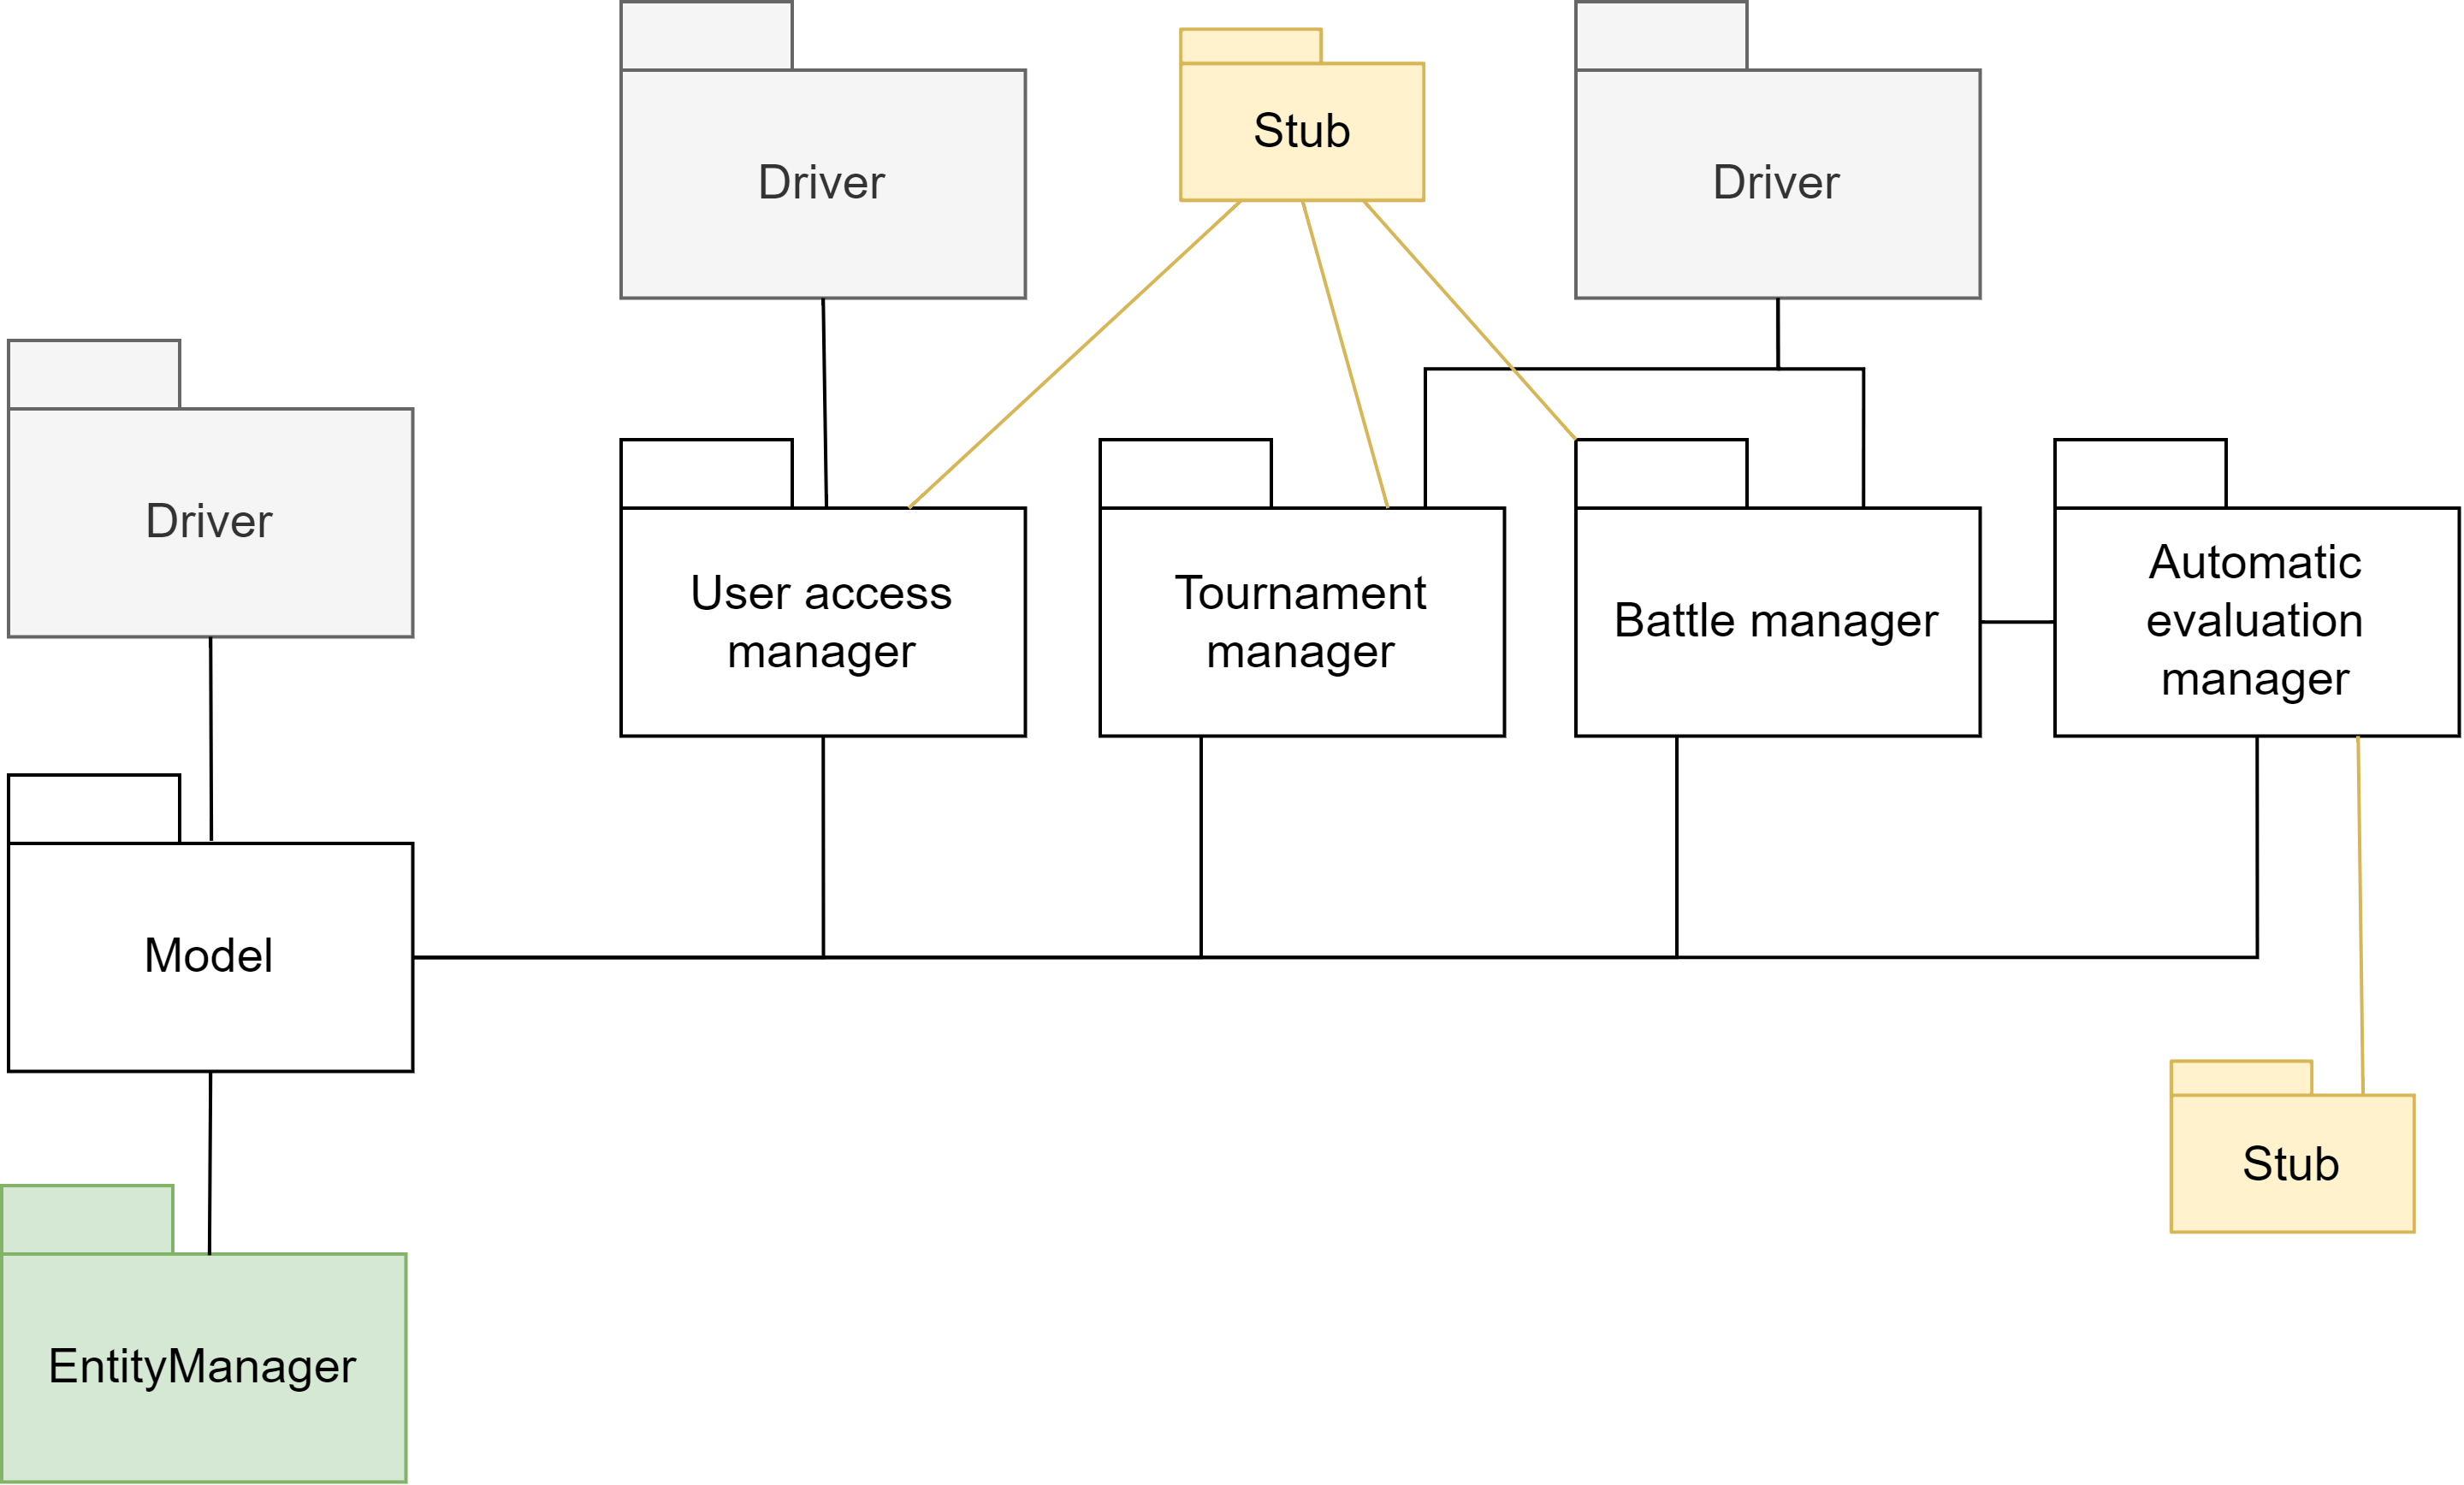
\includegraphics[scale=0.7]{images/testing/stage4.png}
    \caption{Stage 4}
    \label{fig:stage4}
\end{figure}

In the fifth stage (in figure \ref{fig:stage5}) the Mail Manager component is implemented and unit tested. In this way the entire CKB system is working, only the user interfaces are missing.
\begin{figure}[h]
    \centering
    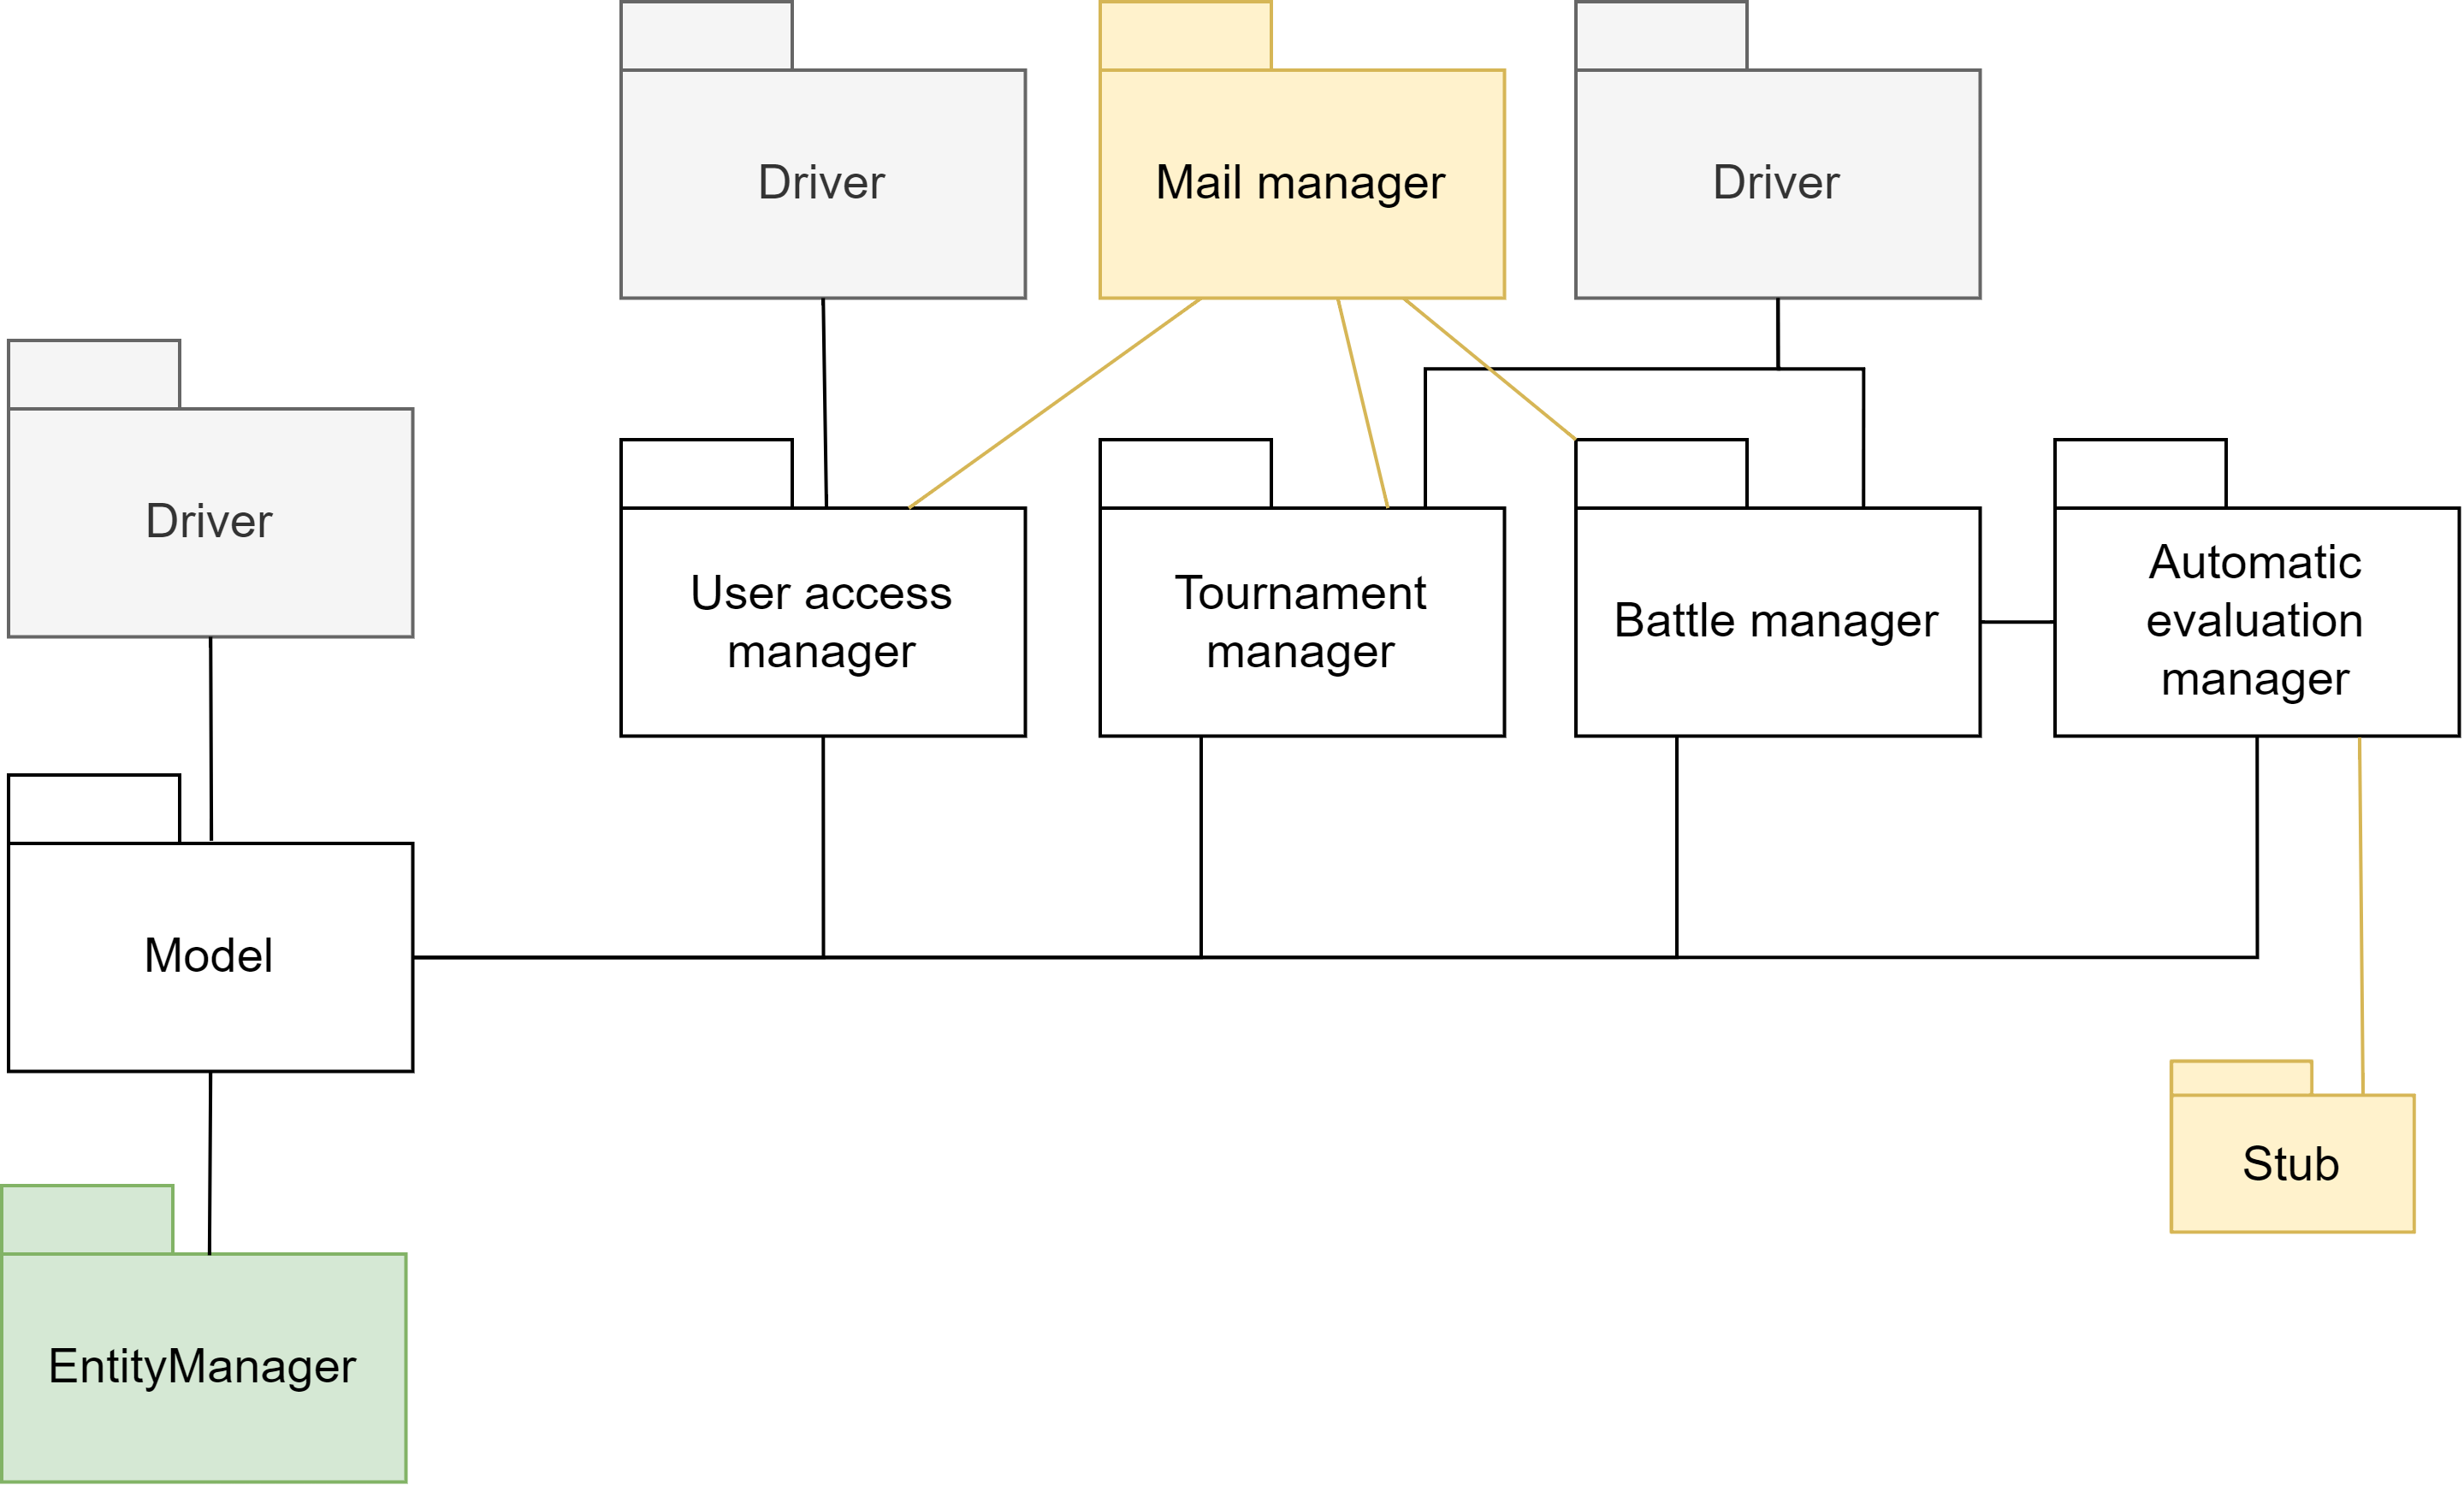
\includegraphics[scale=0.7]{images/testing/stage5.png}
    \caption{Stage 5}
    \label{fig:stage5}
\end{figure}

In the sixth stage (in figure \ref{fig:stage6}), now that all CKB system is working properly, the Dashboard Manager is implemented and tested, as well as the CKB web platform. The whole system has been implemented.
\begin{figure}[h]
    \centering
    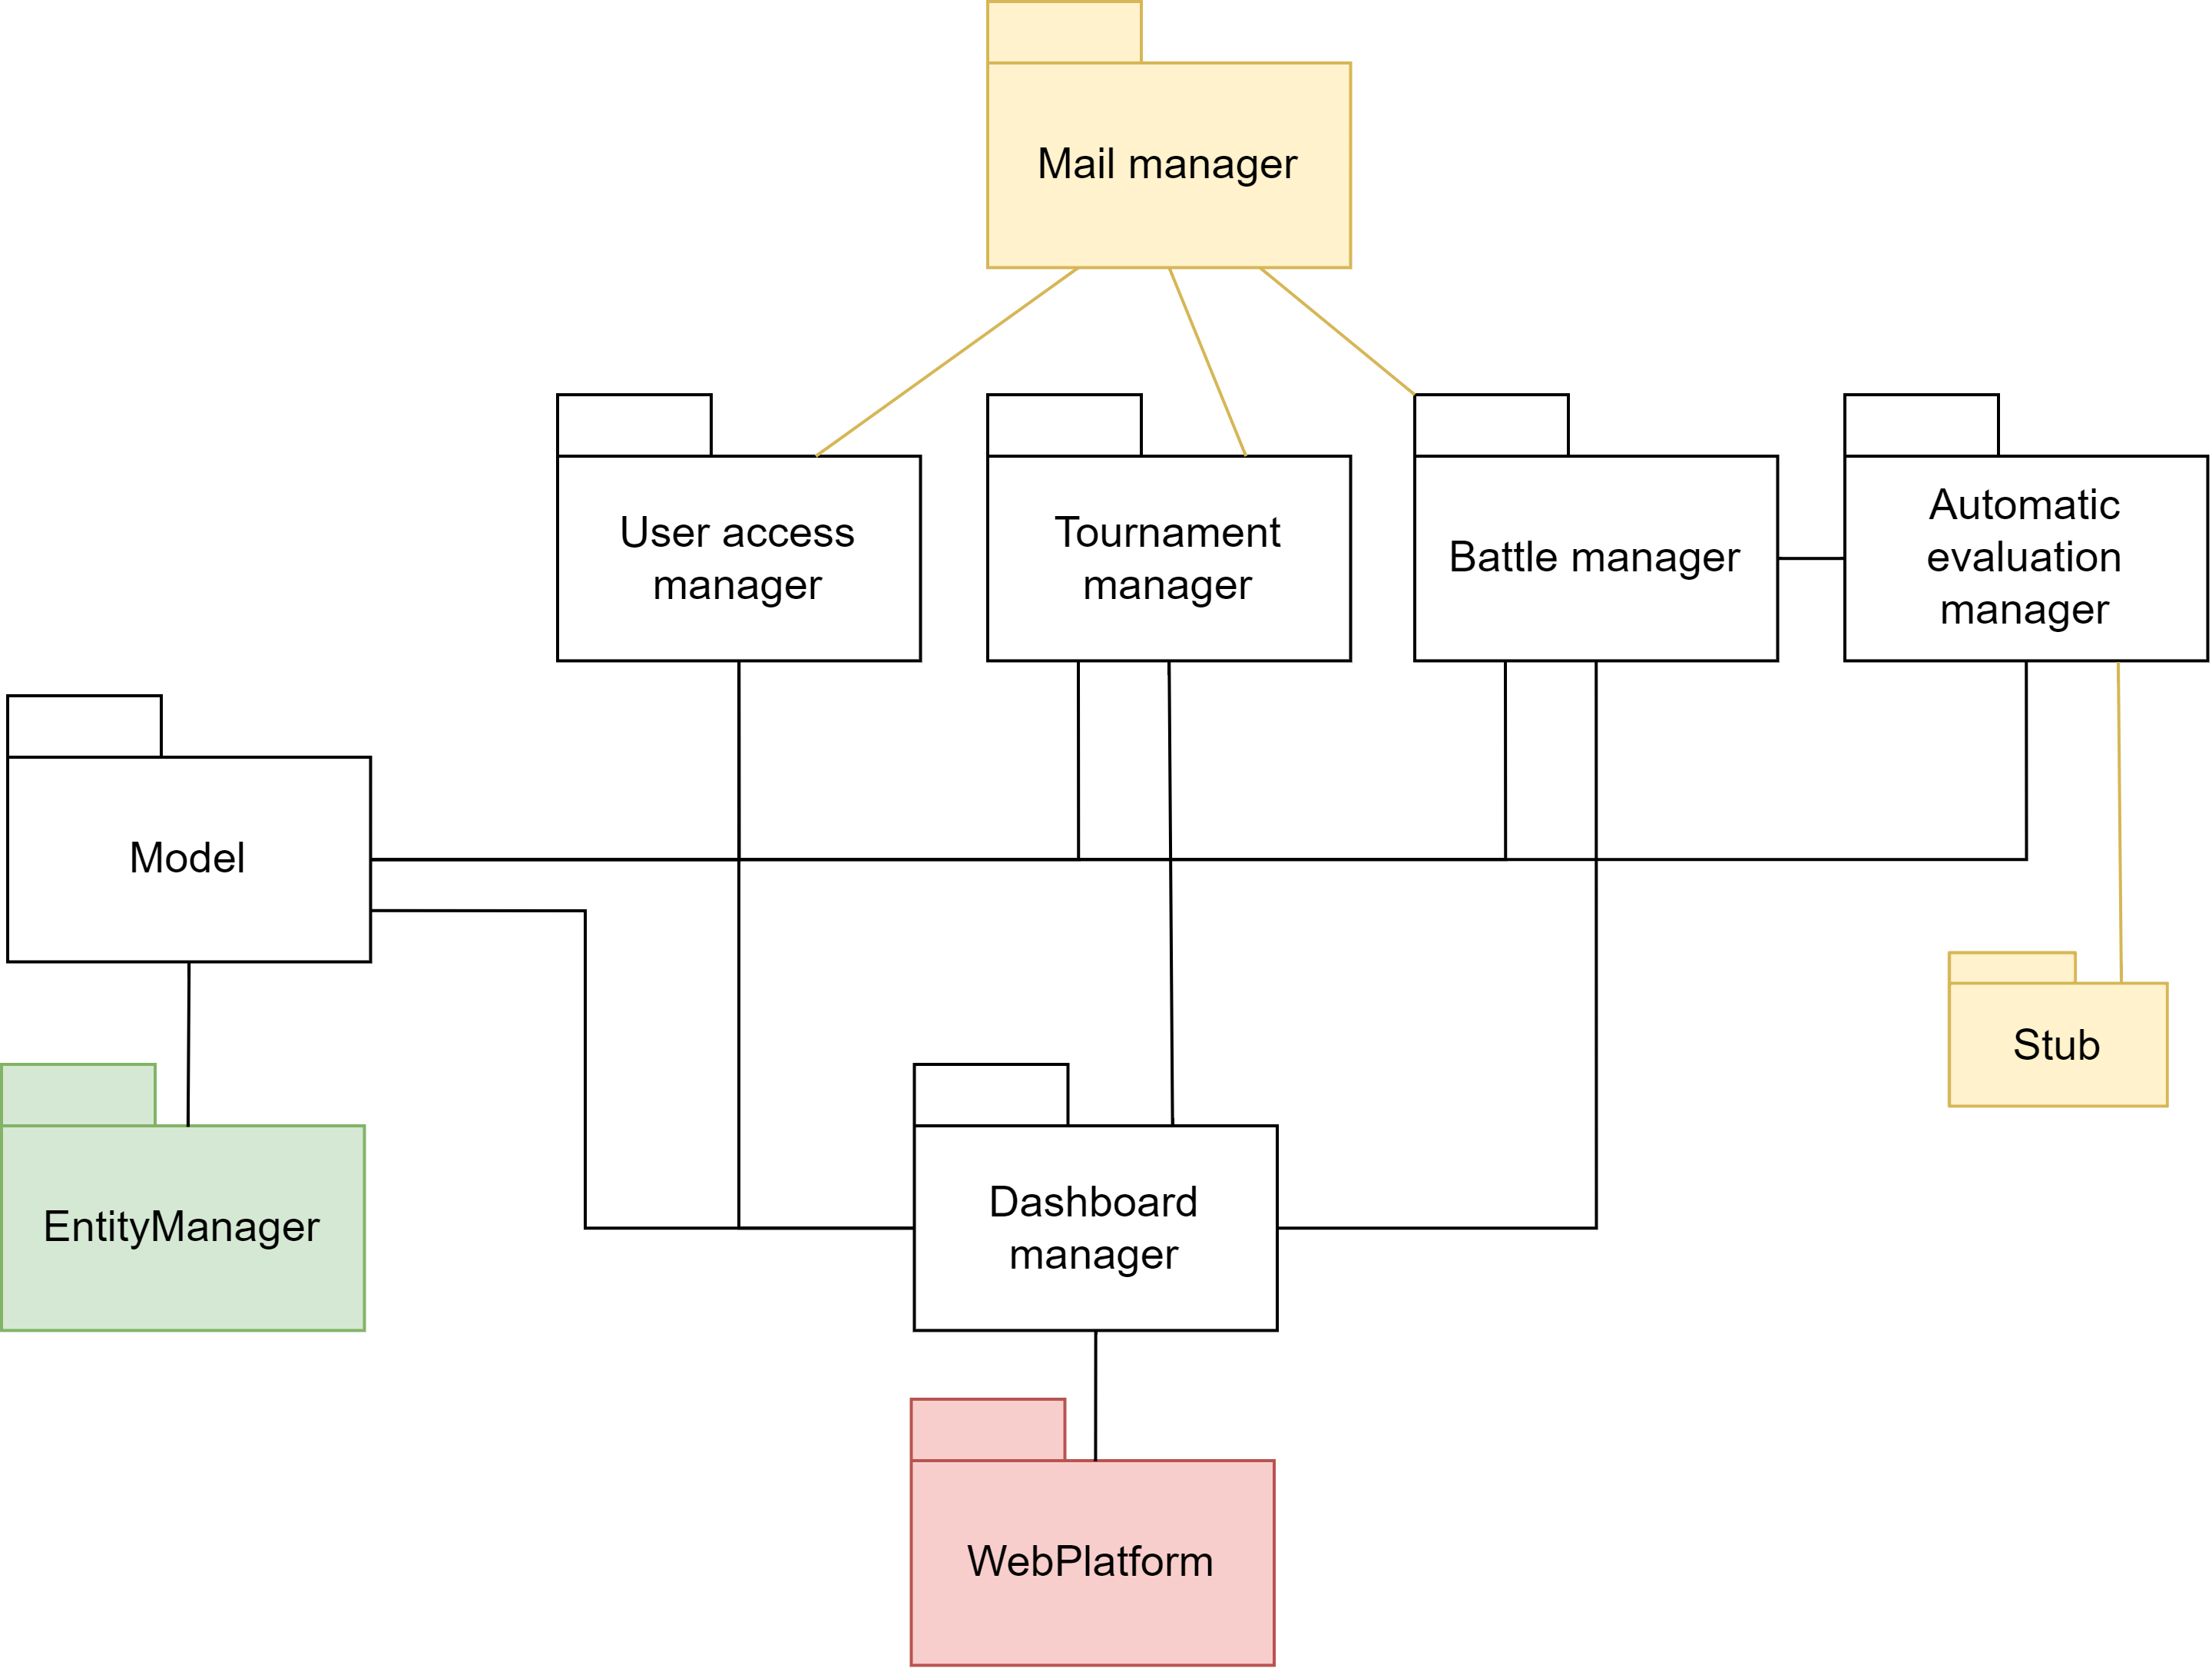
\includegraphics[scale=0.7]{images/testing/stage6.png}
    \caption{Stage 6}
    \label{fig:stage6}
\end{figure}

\section{System testing}\label{sec:systemtesting}
Once the CKB system has been implemented and unit tested, it is important that the system will be tested as a whole in order to verify that all features works well. \newline
Since it is considered that external services are reliable, they do not need to be tested. \newline

Initially, an alpha test of the CKB system will be conducted by the developers in their production environment. A large number of test cases covering at least 80\% of the code will be used to verify all functionalities.
The system testing is composed of the following testing steps:
\begin{itemize}
    \item \textbf{Integration testing}: to ensure that the integration of the CKB system with the external services works correctly. 
    \item \textbf{Functional testing}: to verify that the system meets the functional requirements stated in the RASD.
    \item \textbf{Acceptance testing}: to verify that the system meets the users requirements. It simulates the entire user flow, from both the educator and student view.
    \item \textbf{Security testing}: to identify potential security vulnerabilities.
    \item \textbf{Performance testing}: to evaluate the system performance and response under load. The purpose is to spot any inefficiencies that may affect the system's performance. 
    \item \textbf{Usability testing}: to ensure that the user interface is intuitive and user-friendly (regarding the web platform).
    \item \textbf{Stress testing}: to verify that the system can recover gracefully after a failure. It simulates data loss and the restoration of the system as well as stressful or high-load conditions.
\end{itemize}

At this stage the CKB system should be as close as as possible to the final product. Subsequently a beta test will be executed with the support of a group of voluntary educators and students that will try the web platform independently, and send reports to the developers. This is important in order to verify the correct behavior of the system in a real environment.

\section{Additional specifications on testing}
Every time a new feature is added, the CKB system needs to be tested to check the presence of bugs. In addition, the system testing described in section \ref{sec:systemtesting} has to be performed to confirm that the system as a whole is correct. \newline
During the development of the system it is important to receive regular feedback from stakeholders and users. In this way the correctness of the system is guaranteed along the creation.
